% vim: set textwidth=78 autoindent:
    
\subsection{Using the Delimited Text Plugin}\label{label_dltext}    

The Delimited Text plugin allows you to load a delimited text file  as a layer
in QGIS. 
    
\subsubsection{Requirements}

To view a delimited text file as layer, the text file must contain:

\begin{enumerate}      
\item A delimited header row of field names. This must be the first line in
the text file     
\item The header row must contain an X and Y field. These fields can have any
name.
\item The x and y coordinates must be specified as a number. The coordinate
system is not important
\end{enumerate}

An example of a valid text file might look like this:

\begin{verbatim} 
name|latdec|longdec|cell|
196 mile creek|61.89806|-150.0775|tyonek d-1 ne|
197 1/2 mile creek|61.89472|-150.09972|tyonek d-1 ne|
a b mountain|59.52889|-135.28333|skagway c-1 sw|
apw dam number 2|60.53|-145.75167|cordova c-5 sw|
apw reservoir|60.53167|-145.75333|cordova c-5 sw|
apw reservoir|60.53|-145.75167|cordova c-5 sw|
aaron creek|56.37861|-131.96556|bradfield canal b-6|
aaron island|58.43778|-134.81944|juneau b-3 ne|
aats bay|55.905|-134.24639|craig d-7|
\end{verbatim}


Some items of note about the text file are:

\begin{enumerate}        
\item  The example text file uses \mbox{$|$} as delimiter. Any character can
be used to delimit the fields.
\item The first row is the header row. It contains the fields name, latdec,
longdec, and cell
\item No quotes ({\tt{}"{}}) are used to delimit text fields
\item The x coordinates are contained in the {\em longdec} field
\item The y coordinates are contained in the {\em latdec} field
\end{enumerate}

\subsubsection{Using the Plugin}
To use the plugin you must have QGIS running and use the Plugin Manager to
load the plugin:

Start QGIS, then Open the Plugin Manager by choosing the {\em
Tools\mbox{$|$}Plugin Manager} menu. The Plugin Manager displays a list of
available plugins. Plugins that are already loaded have a check mark to the
left of their name. Click on the checkbox to the left of the {\em Add
Delimited Text Layer} plugin and click Ok to load it as described in Section
\ref{sec:managing_plugins}.


A new toolbar icon is now present:

\includegraphics[width=0.7cm]{toolbar_icon}
Click on the icon to open the Delimited Text dialog as shown in Figure
\ref{fig:delim_text_plugin_dialog}.

\begin{figure}[ht]
   \begin{center}
   \caption{Delimited Text
Dialog}\label{fig:delim_text_plugin_dialog}\smallskip
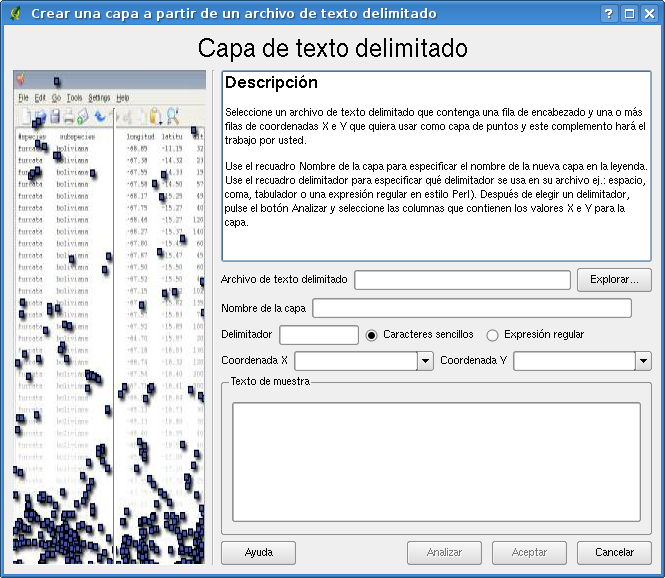
\includegraphics[clip=true, width=8cm]{dialog}            
   \end{center}  
\end{figure}

First select the file to import by clicking on the ellipsis button: 
\includegraphics[scale=0.5]{ellipsis}
Select the desired text file from the file dialog
Once the file is selected, the plugin attempts to parse the file using the
last used delimiter, in this case \mbox{$|$} (see Figure
\ref{fig:delim_text_file_selected}).

\begin{figure}[ht]
   \begin{center}
   \caption{File Selected}\label{fig:delim_text_file_selected}\smallskip
\includegraphics[clip=true, width=8cm]{file_selected}   
   \end{center}  
\end{figure}
  
In this case the delimiter \mbox{$|$} is not correct for the file. The file is
actually tab delimited. Note that the X and Y field drop down boxes do not
contain valid field names.

\begin{figure}[ht]
   \begin{center}
   \caption{Fields Parsed from Text
File}\label{fig:delim_text_file_selected2}\smallskip  
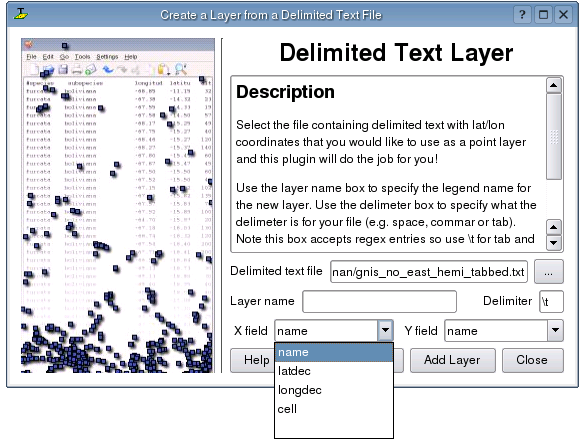
\includegraphics[clip=true, width=8cm]{file_selected2}
   \end{center}  
\end{figure}

To properly parse the file, change the delimiter to
tab using \mbox{$\backslash$}t (this is a regular expression for the tab
character). After changing the delimiter, click {\em Parse}.
The drop down boxes now contain the fields properly parsed as shown in Figure
\ref{fig:delim_text_file_selected2}.

\begin{figure}[ht]
   \begin{center}
   \caption{Selecting the X and Y
Fields}\label{fig:delim_text_file_selected3}\smallskip
\includegraphics[clip=true, width=8cm]{file_selected3}
   \end{center}  
\end{figure}

Choose the X and Y fields from the drop
down boxes and enter a Layer name as shown in Figure
\ref{fig:delim_text_file_selected3}. To add the layer to the
map, click {\em Add Layer}. The delimited text file now behaves as any other
map layer in QGIS.

% html: End of file: `index.html'
